\documentclass[svgnames,tikz]{standalone}
\usetikzlibrary{positioning,backgrounds,calc}

\begin{document}
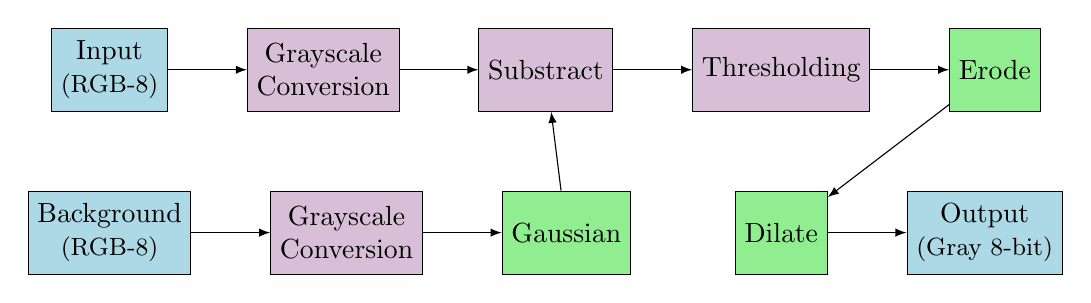
\begin{tikzpicture}
  \tikzset{
    Box/.style={draw, align=center, minimum height=30pt},
    TitleBox/.style={Box, fill=LightGray},
    ImageBox/.style={Box, fill=LightBlue},
    ViewBox/.style={Box, fill=Thistle},
    AlgoBox/.style={Box, fill=LightGreen}
  };


  \node[ImageBox] (A0) []            {Input\\ \small (RGB-8)};
  \node[ViewBox]  (A1) [right=of A0] {Grayscale\\Conversion};
  \node[ViewBox]  (A2) [right=of A1] {Substract};
  \node[ViewBox]  (A3) [right=of A2] {Thresholding};
  \node[AlgoBox]  (A4) [right=of A3] {Erode};
  \node[AlgoBox]  (A5) [below=of A3] {Dilate};
  \node[ImageBox] (A6) [right=of A5] {Output\\ \small (Gray 8-bit)};

  \node[ImageBox] (A7) [below=of A0] {Background\\ \small (RGB-8)};
  \node[ViewBox]  (A8) [right=of A7] {Grayscale\\Conversion};
  \node[AlgoBox]  (A9) [right=of A8] {Gaussian};

  \draw[-latex] (A0) -- (A1);
  \draw[-latex] (A1) -- (A2);
  \draw[-latex] (A2) -- (A3);
  \draw[-latex] (A3) -- (A4);
  \draw[-latex] (A4) -- (A5);
  \draw[-latex] (A5) -- (A6);

  \draw[-latex] (A7) -- (A8);
  \draw[-latex] (A8) -- (A9);
  \draw[-latex] (A9) -- (A2);


  % \draw[DarkGreen, very thick] ($ (A1.north east) + (.48,.5) $)
  %   node [DarkGreen, above left] {Algorithms}
  %   rectangle ($ (A7.south west) + (-.5,-.25) $);


  % \draw[Magenta, very thick] ($ (A2.south west) + (-.48,-.5) $)
  %   node [Magenta, below right] {Views}
  %   rectangle ($ (A4.north east) + (.5,.5) $);

  % \begin{scope}[on background layer]
  %   \fill[LightGray] ($ (A1.north east) + (.48,.5) $) rectangle ($ (A7.south west) + (-.5,-.25) $);
  %   \fill[DarkRed,opacity=0.25] ($ (A2.south west) + (-.48,-.5) $) rectangle ($ (A4.north east) + (.5,.5) $);
  % \end{scope}

\end{tikzpicture}
\end{document}
